\section{Ejercicio 7}

\subsection{El scheduler}

El scheduler mantiene una lista de las tareas vivas y, cada vez que se llama a $sched_proxima_tarea$,
selecciona el próximo candidato a correr.

El enunciado pedía que se devuelva un índice a la gdt con el descriptor de TSS de la tarea,
pero consideramos que sería mas cómodo devolver el tipo y número de la tarea, para que luego
la lógica del juego sepa fácilmente quién está corriendo en el momento.

Para decidir el siguiente elemento se realiza un algoritmo Round-Robin para los grupos y
para las tareas dentro de cada uno.

\subsection{Syscalls}
\label{syscalls}

Las tareas pueden ejecutar varios syscalls a través de la interrupción 0x66,
pasando su código en $eax$.

Los tres syscalls disponibles son:

\begin{itemize}
    \item DONDE (código 0x124) - La tarea pasa como parámetro un puntero a dónde
        el kernel escribe sus coordenadas en el mapa.
    \item SOY (código 0xA6A) - La tarea informa su estado actual,
        pasa como parámetro un código indicando si es Roja, Azul o Neutral.
    \item MAPEAR (código 0xFF3) - La tarea pide al kernel que le mapee una posición xy en el mapa.

        El kernel se encarga de mapear en la página virtual $0x08001000$ de la tarea
        la página física solicitada, con permisos de usuario y escritura.
\end{itemize}

Al finalizar la syscall, la tarea pierde su turno de ejecución.

\subsection{Cambio de tareas}

Cuando una tarea pierde su turno, el kernel pasa a ejecutar la tarea Idle.

Si durante la ejecución de una tarea se produce una excepción
o ella intenta hacer una syscall con parámetros inválidos,
el kernel la marca como muerta (le indica al scheduler que ya no la debe ejecutar)
y pasa a ejecutar la tarea Idle.

Cuando interrumpe el RTC, el kernel le pide al scheduler cuál es la siguiente tarea
a ejecutar y cambia a ella (si es diferente a la actual).

Para hacer estos cambios de tareas llamamos a la función $tss\_switch\_task$ con el
selector del segmento tss a usar. Esta función realiza un $jmp far$ a una dirección
con en el segmento especificado, lo que activa el mecanismo de cambio de tarea del
procesador, que corre el siguiente código.

\begin{lstlisting}
offset: dd 0
selector: dw 0

; void tss_switch_task(short descriptor)
tss_switch_task:
    movzx eax, word [esp+4]
    mov [selector], ax
    jmp far [offset]
    ret
\end{lstlisting}

\subsection{Debugger}
\label{dbg}
El debugger es una herramienta a la hora de programar las tareas, que nos permite ver el estado
de los registros cuando una tarea se muere.

\begin{figure}[H]
    \centering
    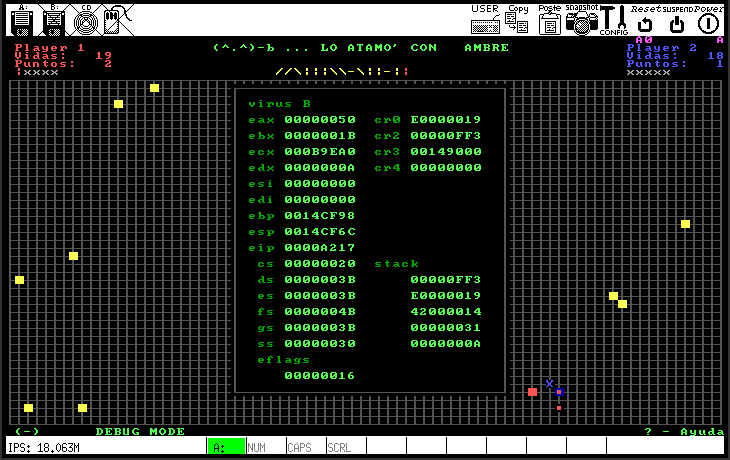
\includegraphics[width=\textwidth]{debugger}
    \caption{Cuadro de información del debugger}
    \label{fig:gates}
\end{figure}

Cuando se mata a una tarea, si está habilitado el modo debug,
se llama a $screen\_show\_debug$.
Esta función recopila el estado actual de los registros y los imprime en pantalla,
junto a el tope del stack.
